\chapter{Идентификация системы связанных релаксационных генераторов}

\section{Реласкационные генераторы: применение, модели}

Применение: собственно генераторы, источники питания.

Элементная база, задачи. Почему возможны хаотические режимы

Не совсем прототип: Kennedy


\cite{mishenko_du_small_relax}

\section{Система из трёх связанных релаксационных генераторов на паре комплиментарных транзисторов}

Основы

\begin{figure}[htb!]
  \centerline{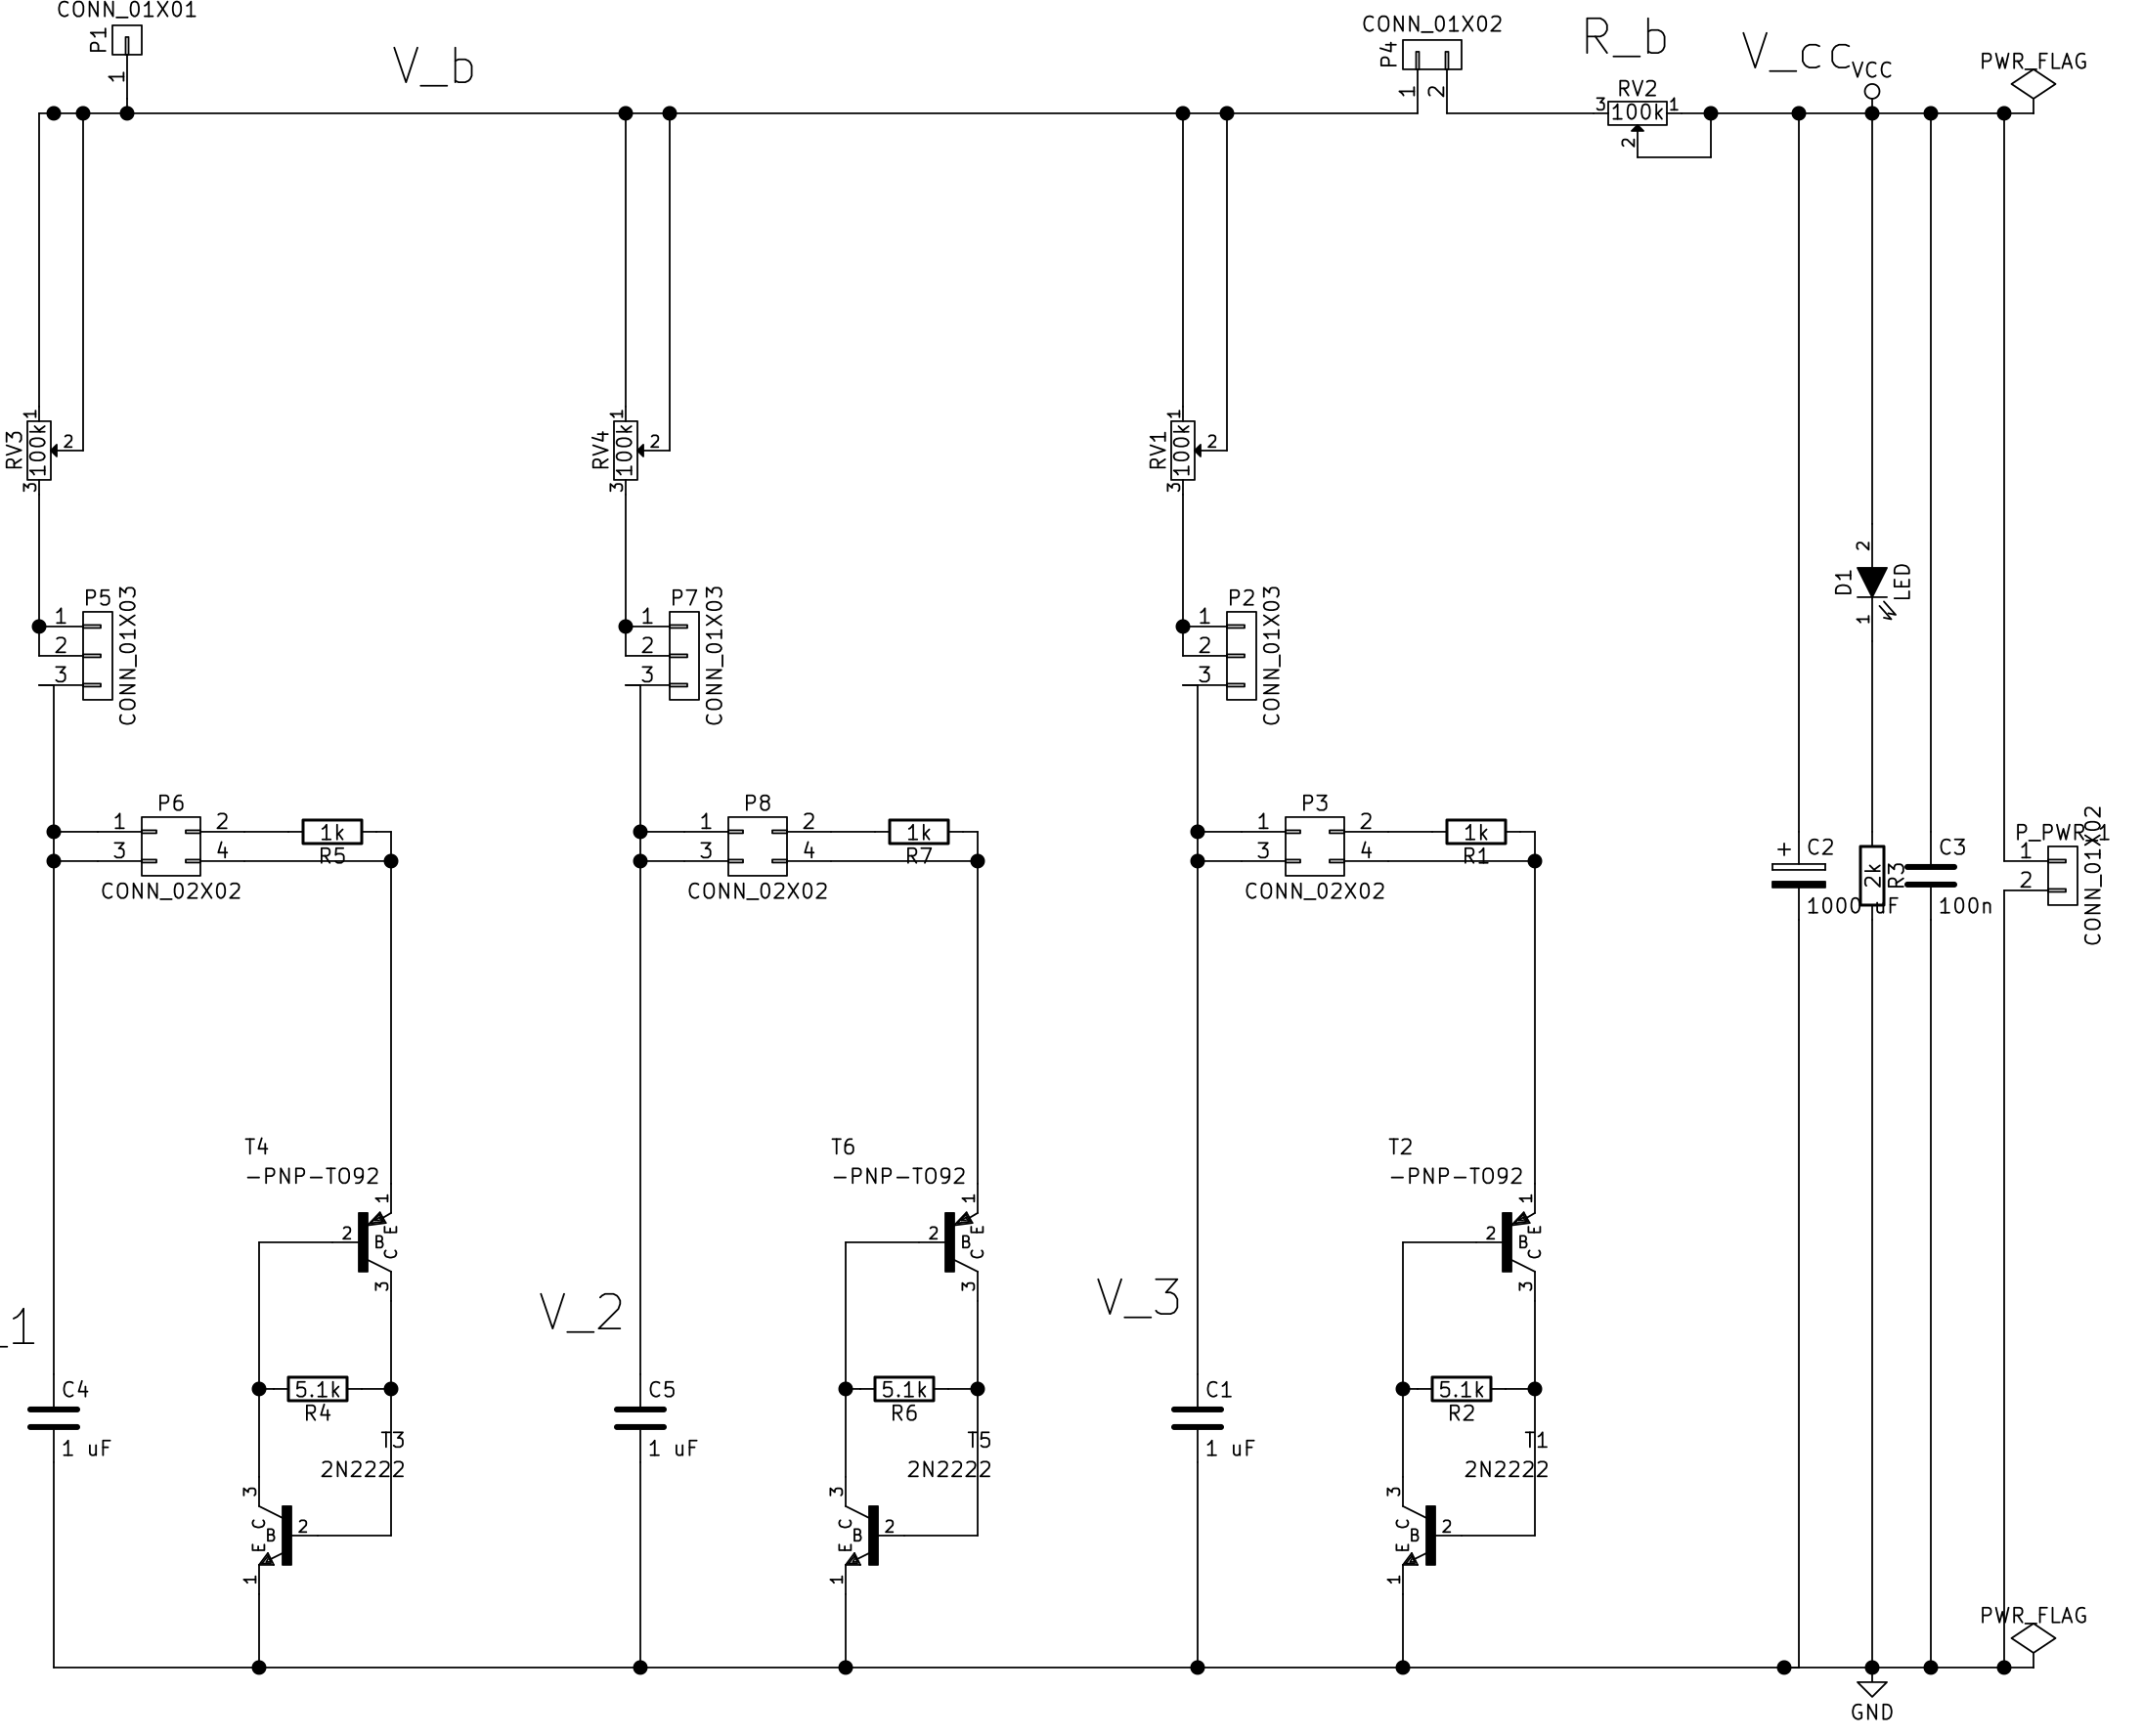
\includegraphics[width=0.7\textwidth]{p/relax3_schem.png} }
  \caption{Электрическая схема системы из трёх связанных релаксационных генераторов на паре комплиментарных транзисторов}
  \label{atu:relax3d_schem}
\end{figure}

Динамика.

\section{Система из трёх связанных релаксационных генераторов на основе триггеров Шмидта}


\section{Модели систем из трёх связанных релаксационных генераторов}


\section{Критерии идентификации систем из трёх связанных релаксационных генераторов}

\section{Идентификация параметра системы из трёх связанных релаксационных генераторов}

\section{Выводы по разделу \thechapter}

Выводы.

